\documentclass[]{report}
\usepackage{amsmath}
\usepackage{amsfonts}
\usepackage{physics}
\usepackage{graphicx}

% Title Page
\title{Symmetry Group Equivariant Neural Networks for Physical Systems}
\author{Alexander J. Heilman}


\begin{document}
\maketitle

\begin{abstract}
a
\end{abstract}

\tableofcontents

\chapter{Introduction: Machine Learning Applied to Materials Science}
The fundamental assumption in any mathematical model of a physical system is that some initial set of properties describing the state of a system fully determines it's future state. 

Physics is essentially the pursuit of rigorous mathematical models that accurately describe physical phenomena. Often these models of physics have some rationale behind them from which they are derived, but such models must always describe the data collected empirically.

Machine Learning (ML) describes a set of techniques which also assume there exists a map between some input space and some target property (though, perhaps, in an extremely complex manner). However, ML approaches generally start with some randomly-chosen but tunable model which is then iteratively tuned or 'trained' to better fit the data directly.
\[
\lbrace \nu_i\rbrace \rightarrow t
\]
	
\chapter{Background: Groups}
A group $G$ is a set with a binary, associative product defined between it's elements under which it is closed, and for which every element, there exists an inverse element (and which also contains an identity element).


\section{Hamiltonian Group}
Consider a physical system that obeys some particular Hamiltonian $H$ with eigenfunctions $\psi^{(i)}(\vec{r})$ and eigenvalues $E^{(i)}$.
$$
H\psi^{(i)}(\vec{r})=E^{(i)}\psi^{(i)}(\vec{r})
$$
Now, we define the group of this Hamiltionian $\mathcal{H}$ to be the group of all operations $h_j \in \mathcal{H}$ with representations (generally reducible) $\mathcal{O}(h_j)$ that leave $H$ invariant when acting on it's input space $\vec{r}$ so that:
$$
H(\mathcal{O}(h_j)\vec{r}) = H(\vec{r})
$$
In this case, the group representations $\mathcal{O}$ acting on the input space $\vec{r}$ can be seen to commute with $H$, in which case they must have simultaneous eigenfunctions $\psi(\vec{r})$.
$$
[H,O]=0 \quad \Rightarrow \quad \mathcal{O}(h_j)H\psi^{(i)}(\vec{r}) = E_i\psi^{(i)}(\vec{r})
$$ 


\section{Representations of Groups}
A group representation $\rho:G\rightarrow GL(V)$ is a map from a set of group elements $G$ to a set of elements in the general linear group $GL(V)$ over a vector space $V$, which preserves group multiplication in cases of composition in $GL(V)$. In general, maps that preserve the action of the group in the codomain are referred to as homomorphisms.

A faithful representation is one which acts as a bijection, that is, each group element gets mapped to a unique element in the representation space. Every group has at least one representation, the trivial representation, which maps every group element to the number 1, so that the group multiplication is trivially preserved; however, the trivial representation is clearly not faithful. Finite order groups always admit at least one faithful representation, the regular representation, which maps each element to a corresponding permutation matrix. However, this representation space (of size $N\times N$, where $N$ is the order of the group) is rather large. Often, groups admit smaller representations, which leads to considerations of whether there exist `atomic' or smallest representation, which are referred to as irreducible representations.


\subsection{Irreducible Representations}
Irreducible representations essentially act as the building blocks of all possible representations of a group. In general, a representation $\rho$ is decomposable as a direct sum of irreducible representations $\Gamma^{(\alpha)}$ as:
\begin{equation}
\rho = \bigoplus_{\alpha}c_{\alpha}\Gamma^{(\alpha)}
\end{equation}
where $\alpha$ indexes the irreducible representations of the group and the expansion coefficient $c_{\alpha}$ is some positive integer. The coefficient of this expansion is derivable from the characters of $\rho$ and $\Gamma^{(\alpha)}$ as:
\begin{equation}
c_{\alpha}=\frac{1}{N}\sum_{g\in G}\big[\chi^{(\alpha)}(g)\big]^*\chi(g)
\end{equation}
The number of irreducible representations $n_{\Gamma}$ of a group is equal to the number of equivalence classes of a group $n_c$.
\begin{equation}
n_{\Gamma}=n_c
\end{equation}
Furthermore, the sum of the squares of the dimensions of the irreducible representations $d_{\alpha}$ is equal to the number of group elements $N$ as:
\begin{equation}
	N = \sum_{\alpha}d_{\alpha}^2
\end{equation}


\subsection{Characters}
The explicit form of a representation is, in general, dependent upon a particular choice of basis and thus hard to characterize universally. The trace of a matrix, however, is invariant under change of basis. This motivates the definition of the character $\chi^{\alpha}(g)$ of a representation $\Gamma^{(\alpha)}$ for group element $g$, defined as:
\begin{equation}
	\chi^{\alpha}(g)=\text{Tr}\Big[\Gamma^{(\alpha)}(g)\Big]
\end{equation}
The characters are basis-independent by construction and allow one to universally characterize the representations of a group.
	
\section{Basis Functions}
The general linear group $GL(V):V\rightarrow V$ is the set of linear operators acting on the vector space $V$. Group representations map elements $g\in G$ to elements $M\in GL(V)$, which have a natural action on the underlying vector space $V$.

\subsection{SO(3) Basis Functions}
Spherical harmonics $Y_{\ell}^m$ are a set of functions that form a basis for functions on the surface of a sphere, analogous to the sinusoidal functions correspondence to a plane.

\subsection{Irreducible Representations of Permutation Groups}
The irreducible representations of the permutation (or symmetric) Groups $S_n$ may be represented and cataloged diagrammatically with a set of objects known as Young Diagrams. From these diagrams, we may further construct symmetrizers which act as projection operators for relevant basis sets. 

\subsubsection{Young Diagrams}
Young diagrams of order $n$ are left-justified arrangements of boxes into $k$ rows stacked vertically in non-increasing order. 
\begin{figure}\centering
	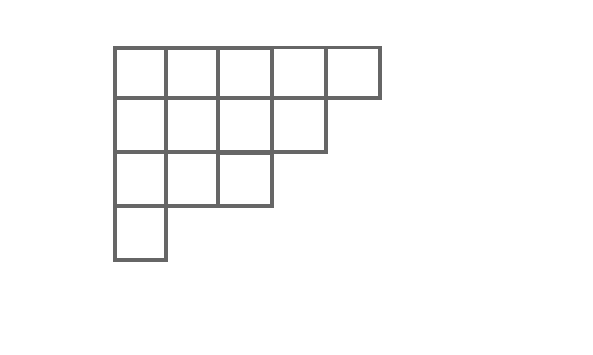
\includegraphics[scale=0.6]{youngdiagram-ex.pdf}
	\caption{Example Young diagram of shape $(5,4,3,1)$.}
\end{figure}
A Young diagram is said to be of some shape $\lambda:(\lambda_1,\lambda_2,...,\lambda_k)$, where $\lambda_i$ refers to the depth of row $i$ and $\lambda_{i+1}\leq\lambda_i\leq\lambda_{i-1}$. 

We can then form a set of Young tableaux from diagrams by filling in the boxes from a set of ordered indices $\lbrace x_1,x_2,...,x_k\rbrace$ corresponding to tensor components $T^{x_1x_2...x_k}$.  A standard tableu is one filled with indices $x_i$ (without repeats) with entries increasing in index $i$ down each column and across (to the right) rows.
\begin{figure}\centering
	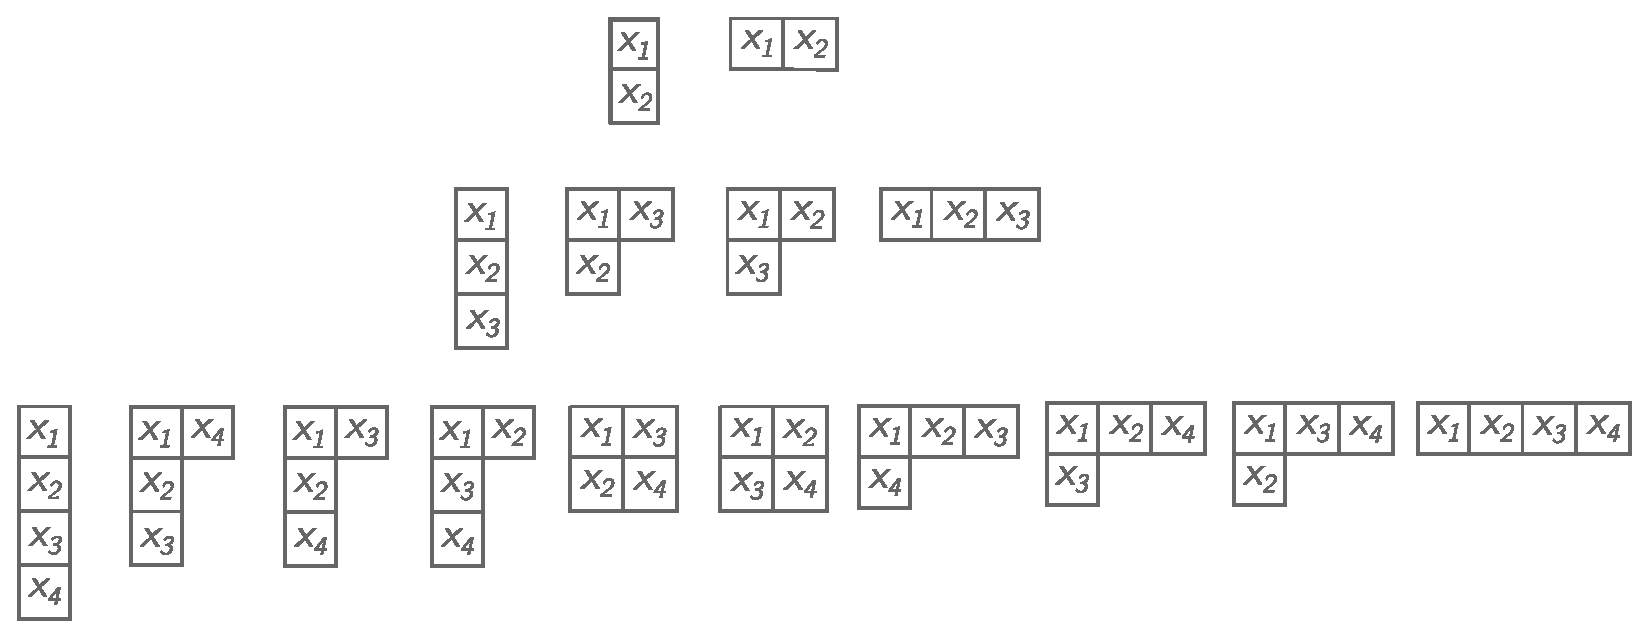
\includegraphics[scale=0.42]{youngtableaux-ex.pdf}
	\caption{Standard Young tableaux for diagrams of at most 4 boxes.}
\end{figure}

Each of these standard tableaux correspond to an invariant subspace under $S_k$. From these tableau, we may construct so-called \textit{Young Symmetrizers}, which project tensors onto their corresponding $S_k$-invariant subspace. 

A Young symmetrizer $P_{\lambda}$ corresponding to tableau $\lambda$ is composed of a compound set of symmetrizing operations $s_{\lambda}$ and antisymmetrizing operations $a_{\lambda}$, scaled by an overall normalization constant $C_{\lambda}$:
$$
P_{\lambda} = \mathcal{C}_{\lambda}s_{\lambda}a_{\lambda}
$$
Where here, we adopt the convention of anti-symmetrization before symmetrization, following that in Itin \cite{Itin-r3}.

The symmetrizing operator $s_{\lambda}$ for a diagram $\lambda$ is composed of a product of symmetrizers $\mathcal{S}(\mathcal{I})$, where $\mathcal{I}$ ranges over all subsets of indices corresponding to some vertically stacked set of indices in tableau $\lambda$, i.e.:
$$
s_{\lambda} = \prod_{\mathcal{I}\in \text{Cols}(\lambda)}\mathcal{S}(\mathcal{I})
$$
where $\text{Cols}(\lambda)$ represents the set of disjoint subsets of indices down each column, and symmetrizers $\mathcal{S}$ are defined to act on tensors $T$ component-wise as:
$$
\big[\mathcal{S}(\mathcal{I})T\big]_{ijk...}= \sum_{\sigma_{\mathcal{I}}}T_{\sigma_{\mathcal{I}}(ijk...)}
$$
where $\sigma_{\mathcal{I}}$ are permutations of index subset $\mathcal{I}$.

Similarly, the antisymmetrizing operator $a_{\lambda}$ can be constructed as a product of antisymmetrizers:
$$
a_{\lambda} = \prod_{\mathcal{I}\in \text{Rows}(\lambda)}\mathcal{A}(\mathcal{I})
$$
where $\text{Rows}(\lambda)$ represents the set of  disjoint subsets of indices across each entire row, and antisymmetrizers $\mathcal{A}$ are defined as:
$$
\big[\mathcal{A}(\mathcal{I})T\big]_{ijk...}= \sum_{\sigma_{\mathcal{I}}}\text{sgn}(\sigma_{\mathcal{I}})T_{\sigma_{\mathcal{I}}(ijk...)}
$$
where, again, $\sigma_{\mathcal{I}}$ range over all permutations of index subset $\mathcal{I}$.



The normalization constant $C_{\lambda}$ may be derived from the shape of the underlying Young diagram according to the \textit{hook-length formula}, given below, where $\text{hook}(\alpha,\beta)$ returns the number of boxes crossed by a hook coming up (from below) column $\beta$ and out of the diagram to the right in row $\alpha$.
$$
C_{\lambda}= \prod_{(\alpha,\beta)\in \lambda}\frac{1}{\text{hook}(\alpha,\beta)}
$$
Furthermore, the number of independent components $N_{\lambda}$ of a tensor subspace corresponding to some Young tableau with shape $\lambda$ may also be derived from the diagram by a related hook-length formula:
$$
N_{\lambda}= \prod_{(\alpha,\beta)\in \lambda}\frac{n-\alpha+\beta}{\text{hook}(\alpha,\beta)}
$$
where $n$ is the dimension of the vector space forming the tensor space. 

Thus, the standard Young tableaux of $k$ boxes can be used to decompose an arbitrary tensor space into a set of $GL$ invariant subspaces with known symmetries (under permutation of indices) by way of corresponding Young symmetrizers. These known symmetries will be relevant in the further decomposition of these subspaces by way of contractions with the metric tensor, and the fully antisymmetric tensor, discussed below.
\begin{figure}\centering
	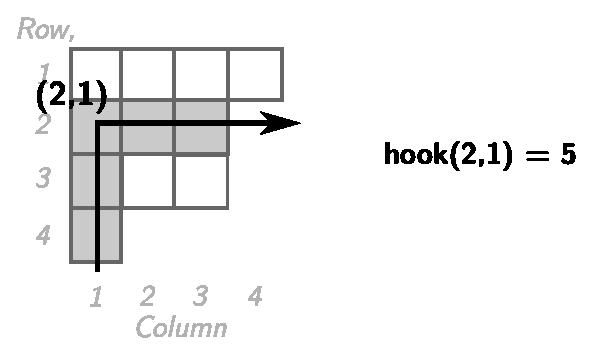
\includegraphics[scale=0.6]{hook-ex.pdf}
	\caption{Example value of $\text{hook}(2,1)$ for a diagram of shape $\lambda:(4,3,3,1)$. Note that it's corresponding normalization constant is $C_{\lambda}=1/33600$.}
\end{figure}

\subsubsection{Schur-Weyl Duality}

Under the joint action of the symmetric group $S_k$ and $GL_n$ acting on a tensor of rank-$k$ over $(\mathbb{C}^n)^{\otimes k}$, the tensor space may be decomposed into a direct sum of tensor products of representations of $S_k$, $\pi_k$ and representations of $GL_n$, here $\rho_n$, simultaneously indexed by the set of Young diagrams $\lambda$ of order $k$. That is,
$$
\underbrace{\mathbb{C}^n\otimes ... \otimes\mathbb{C}^n}_k= \bigoplus_{\lambda}\pi^{(\lambda)}_{k}\otimes\rho_n^{(\lambda)}.
$$
This is a statement of the Schur-Weyl duality without proof. The point here though is that the representations under $GL$ of a complex tensor product space, are indexed by the same set (that is, they both are described by the same underlying structure) as the representations under $S$.  Thus, we consider the $GL$ decomposition to be synonymous here with the symmetric group $S$ decomposition.

\section{Coupling and Clebsch-Gordan Coefficients}


\chapter{Equivariant Graph Neural Networks}


\section{Graph Neural Networks}
Neural networks are a class of universal function approximators, composed layer-wise by functions $\mathcal{L}^1\circ\mathcal{L}^2\circ ... \circ \mathcal{L}^n $, where each layer-to-layer transition map $\mathcal{L}^i$ is a trainable function from some feature space associated with layer $L$ to a feature space associated with layer $L+1$.

Many modern approaches use a specific type of neural network, referred to as a Graph Neural Network (GNN), which act on data encoded in features associated with some representative graph (i.e. a collection of nodes and connections between them).


\subsection{Equivariance}
A function $f:X\rightarrow Y$ is equivariant with respect to a group $G$ if, for representations $\mathcal{D}_X$ and $\mathcal{D}_Y$ of $G$ (over spaces $X$ and $Y$, respectively), it satisfies:
$$
f(D_X(g)x) = D_Y(g)f(x) \quad\quad \forall g\in G
$$
Essentially, a function is equivariant with respect to some group if it 'commutes' with the representations of groups on it's input and output space. 

\subsubsection*{Invariance}
A special case of equivariance then is \textit{invariance}, where the representations of all group elements in the output space are identity (i.e. $D_Y$ is the trivial representation). That is, a function $f:X\rightarrow Y$ is invariant under a group $G$ if it satisfies:
$$
f\circ \mathcal{D}_X(g) = f \quad
\ \forall g\in G.
$$



\chapter{Crystal Group Equivariant Networks}

\medskip

\end{document}          
